\documentclass[12pt,aspectratio=169]{beamer}
\usetheme[version=2024]{iiasa}

\title{MESSAGEix-Transport/-GLOBIOM}
\subtitle{and the 2024 ScenarioMIP/SSP update}
\institute{
  Energy, Climate, and Environment (ECE) Program \\
  International Institute for Applied Systems Analysis (IIASA)}

\date{
  \texorpdfstring{7th International Transport Energy Modeling workshop (iTEM7)\\
  Wed, 18 September 2024}%
  {2024-09-19}}

\author{\texorpdfstring{Paul Kishimoto, Aneeque Javaid, Takuya Hara, Volker~Krey, Bas van Ruijven\\
  \href{mailto:kishimot@iiasa.ac.at}{\ttfamily \scriptsize <kishimot@iiasa.ac.at>}%
  }{Paul Natsuo Kishimoto <kishimot@iiasa.ac.at>}}

\usepackage[
  maxnames = 1,
  style = authoryear,
  giveninits,
  terseinits,
  maxcitenames = 3,
  ]{biblatex}
\addbibresource{all.bib}

\usepackage{minted}

\begin{document}

\maketitle

\begin{frame}
\frametitle{Outline}

\tableofcontents

\end{frame}

\section{MESSAGEix-Transport}

\subsection{Open source, finally}

\begin{frame}
\frametitle{MESSAGEix-Transport code \& data}
\framesubtitle{Open source—finally!}

{\Large
Docs: \href{https://docs.messageix.org/models}{docs.messageix.org/models}

\smallskip
Code \& data: \href{https://github.com/iiasa/message-ix-models}{github.com/iiasa/message-ix-models}

\medskip
Issues and pull requests: \href{https://github.com/search?q=repo\%3Aiiasa\%2Fmessage-ix-models+label\%3Atransport\&type=issues}{(link)}
}

\end{frame}

\subsection{About the model: purpose, requirements, structure}

\begin{frame}[allowframebreaks]
\frametitle{MESSAGEix-GLOBIOM model family}
Linear optimization (LP)-based \structure{integrated assessment models (IAMs)}:
\begin{itemize}
  \item ‘Integrative’ of the full global energy-economic system.
  \item For ‘assessment’ of future scenarios (incl. climate policy) and their effects on \structure{global total emissions}.
  \item Linked to MACRO (CGE), GLOBIOM (land use, via emulator).
  \item Spatial resolution: 12 regions.
  \item Temporal scope \& resolution: 5- and 10-year periods to 2110.
\end{itemize}

\medskip
A \structure{family} because:
\begin{itemize}
  \item Many model \structure{variants} with similar but different structure: spatial scope/res.; sets of technologies; constraints.
  \item e.g. MESSAGEix-Nexus, MESSAGEix-Materials, MESSAGEix-Buildings.
\end{itemize}

\framebreak
\href{https://github.com/iiasa/message-ix-models}{\ttfamily message-ix-models} —a Python package for code to \structure{build} (set up structure + add data) → \structure{solve} → \structure{report} (postprocess) MESSAGEix-GLOBIOM scenarios.
\begin{itemize}
  \item Free and open source since 2021.
  \item 14,000+ lines of Python code; submodules for model variants.
  \item Documentation, changelog, test suite, automated quality control (QC) and validation.
  \item Not \emph{all} MESSAGEix-GLOBIOM applications and code (some still private), but a growing share.
  \item >1 ‘snapshot’ of the base/global MESSAGEix-GLOBIOM available on Zenodo (\href{https://docs.messageix.org/projects/models/en/latest/api/model-snapshot.html}{docs}).
\end{itemize}

\end{frame}

\begin{frame}
\frametitle{MESSAGEix-Transport: a variant in the family}

MESSAGEix-GLOBIOM transport structure is \structure{aggregated/low resolution}.
\begin{itemize}
  \item Technologies like \texttt{t=elec\_trp}: sum total of all transport modes, vehicle types, powertrains that input commodity \texttt{c=electr}.
  \item Input in [GW·a] of (final) energy; output in [GW·a] of ‘useful energy’.
  \item Exogenous%
  \footnote{Aggregate price elasticity via MACRO.}
  \texttt{demand} projection for this useful energy.
\end{itemize}

MESSAGEix-Transport structure is (slightly) \structure{higher resolution}.
\begin{itemize}
  \item Transport \texttt{demand} expressed in PDT [km] or freight volume [t·km], projected using outside calculation, data sources, and models.
  \item Intermediate VDT [km] for 5 passenger and 2 freight modes.
  \item 1-10 technologies for each (service, mode) → distinct costs, efficiencies, constraints. \texttt{CAP}-acity variable measures vehicle stock [10⁶]; \texttt{ACT}-ivity measures VDT [10⁹ km/a].
\end{itemize}
\end{frame}

\begin{frame}
\frametitle{MESSAGEix-Transport}
\framesubtitle{Purpose and applications}

These are most importantly \structure{varied}—this is a tool meant to be used for multiple purposes—but include:
\begin{itemize}
  \item Add transport sector detail to scenarios \& reported/output data while \structure{retain the detail} of MESSAGEix-GLOBIOM's scope \& representation of energy supply, land use, other sectors.
  \item Provide \structure{aggregate outputs to calibrate} the ‘base’ (\texttt{t=elec\_trp}) representation.%
  \footnote{As in ScenarioMIP / SSP (2024)—second half of this talk.}
  \item \structure{Enable connections to transport literature and data}:
  \begin{itemize}
    \item Higher-resolution (if not “bottom-up”) models, e.g. ITF-OECD ‘PASTA’.
    \item Data on stocks; techno-economics of technologies; mode share; etc. that is recognizable to iTEM participants.
  \end{itemize}
\end{itemize}
\end{frame}

\subsection{Development and calibration; \texttt{genno}}
\begin{frame}
\frametitle{Development and calibration}

\begin{itemize}
  \item Initial data and structure from \textcite{mccollum-2017}.
  \item New system for \structure{build} and \structure{report} portions of workflows.
  \item Workflow automation and testing.
\end{itemize}

\medskip
These serve some \structure{process and usability goals}:
\begin{enumerate}
  \item Provide \structure{flexibility} for the varied applications (above),
  \item Enable \structure{repeatable, reproducible} workflows.
  \begin{itemize}
    \item Push-button to rebuild the model from scratch w/ updated data.
    \item Automated ‘nightly’ runs.
  \end{itemize}
  \item Reduce development/maintenance burden and facilitate collaboration.

  (Only <2 FTE working on this implementation).
\end{enumerate}
\end{frame}

\begin{frame}
\frametitle{Implementation detail: input data workflows}

Often in model-building we need to set values of some parameter $C$ derived from other quantities like: $$C_{s,t,n,y} = A \times B$$
\vspace*{-5mm}
\begin{itemize}
  \item with dimensions like ‘s’cenario, ‘t’echnology, ‘n’ode (geo), ‘y’ear/period…
  \item e.g. total VDT [km/a] = vehicle stock [1] × average driving distance per vehicle per year [km/a]
\end{itemize}

BUT! \structure{What are the dimensions of $A$, $B$?}
\begin{itemize}
  \item Often we don't have data at the desired resolution, e.g. only $A_{n,y}$ for a subset of all $y$.
  \item Or, we may apply \structure{assumptions} to produce $B_{s} = k_{s,n,y}(…) × B_{n,t}$.
  \item We may want to change these choices over time.
\end{itemize}

\end{frame}

\begin{frame}[fragile,allowframebreaks]
\frametitle{\texttt{genno}: a library for $N$-D data workflows}

Describe calculations as \structure{atomic operations} in either \emph{dimension-agnostic} or dimensionally precise manner.

\medskip
Generic:
\begin{minted}{python}
c = genno.Computer()
c.eval("""
    Z = - (0.5 / (X ** 3))
    A = X ** 3 + Z
    B = A + A
    D = assign_units(B, "km")
    """)
\end{minted}
Dimensionality and units of derived quantities are inferred automatically.

\framebreak
In MESSAGEix-Transport, this allows to \structure{compose} calibration and input data workflows using \structure{small functions}/steps: \verb@logit@, \verb@mul@, \verb@factor_pdt@
\begin{minted}{python}
# Mode shares
c.add(ms, "logit", cost, sw, "lambda:", y), dict(dim="t")
# Total PDT (n, t, y), with modes for the 't' dimension
c.add(pdt_nyt + "0", "mul", pdt_ny, ms)
# Scenario-specific adjustment factors
c.add("pdt factor:n-y-t", "factor_pdt", n, y, t_modes, "config")
\end{minted}

\medskip
Because small, these are \structure{reusable}, \structure{testable}, easy to document/read (\structure{transparent}), etc.

\framebreak
\begin{columns}
\column[T]{0.6\paperwidth}
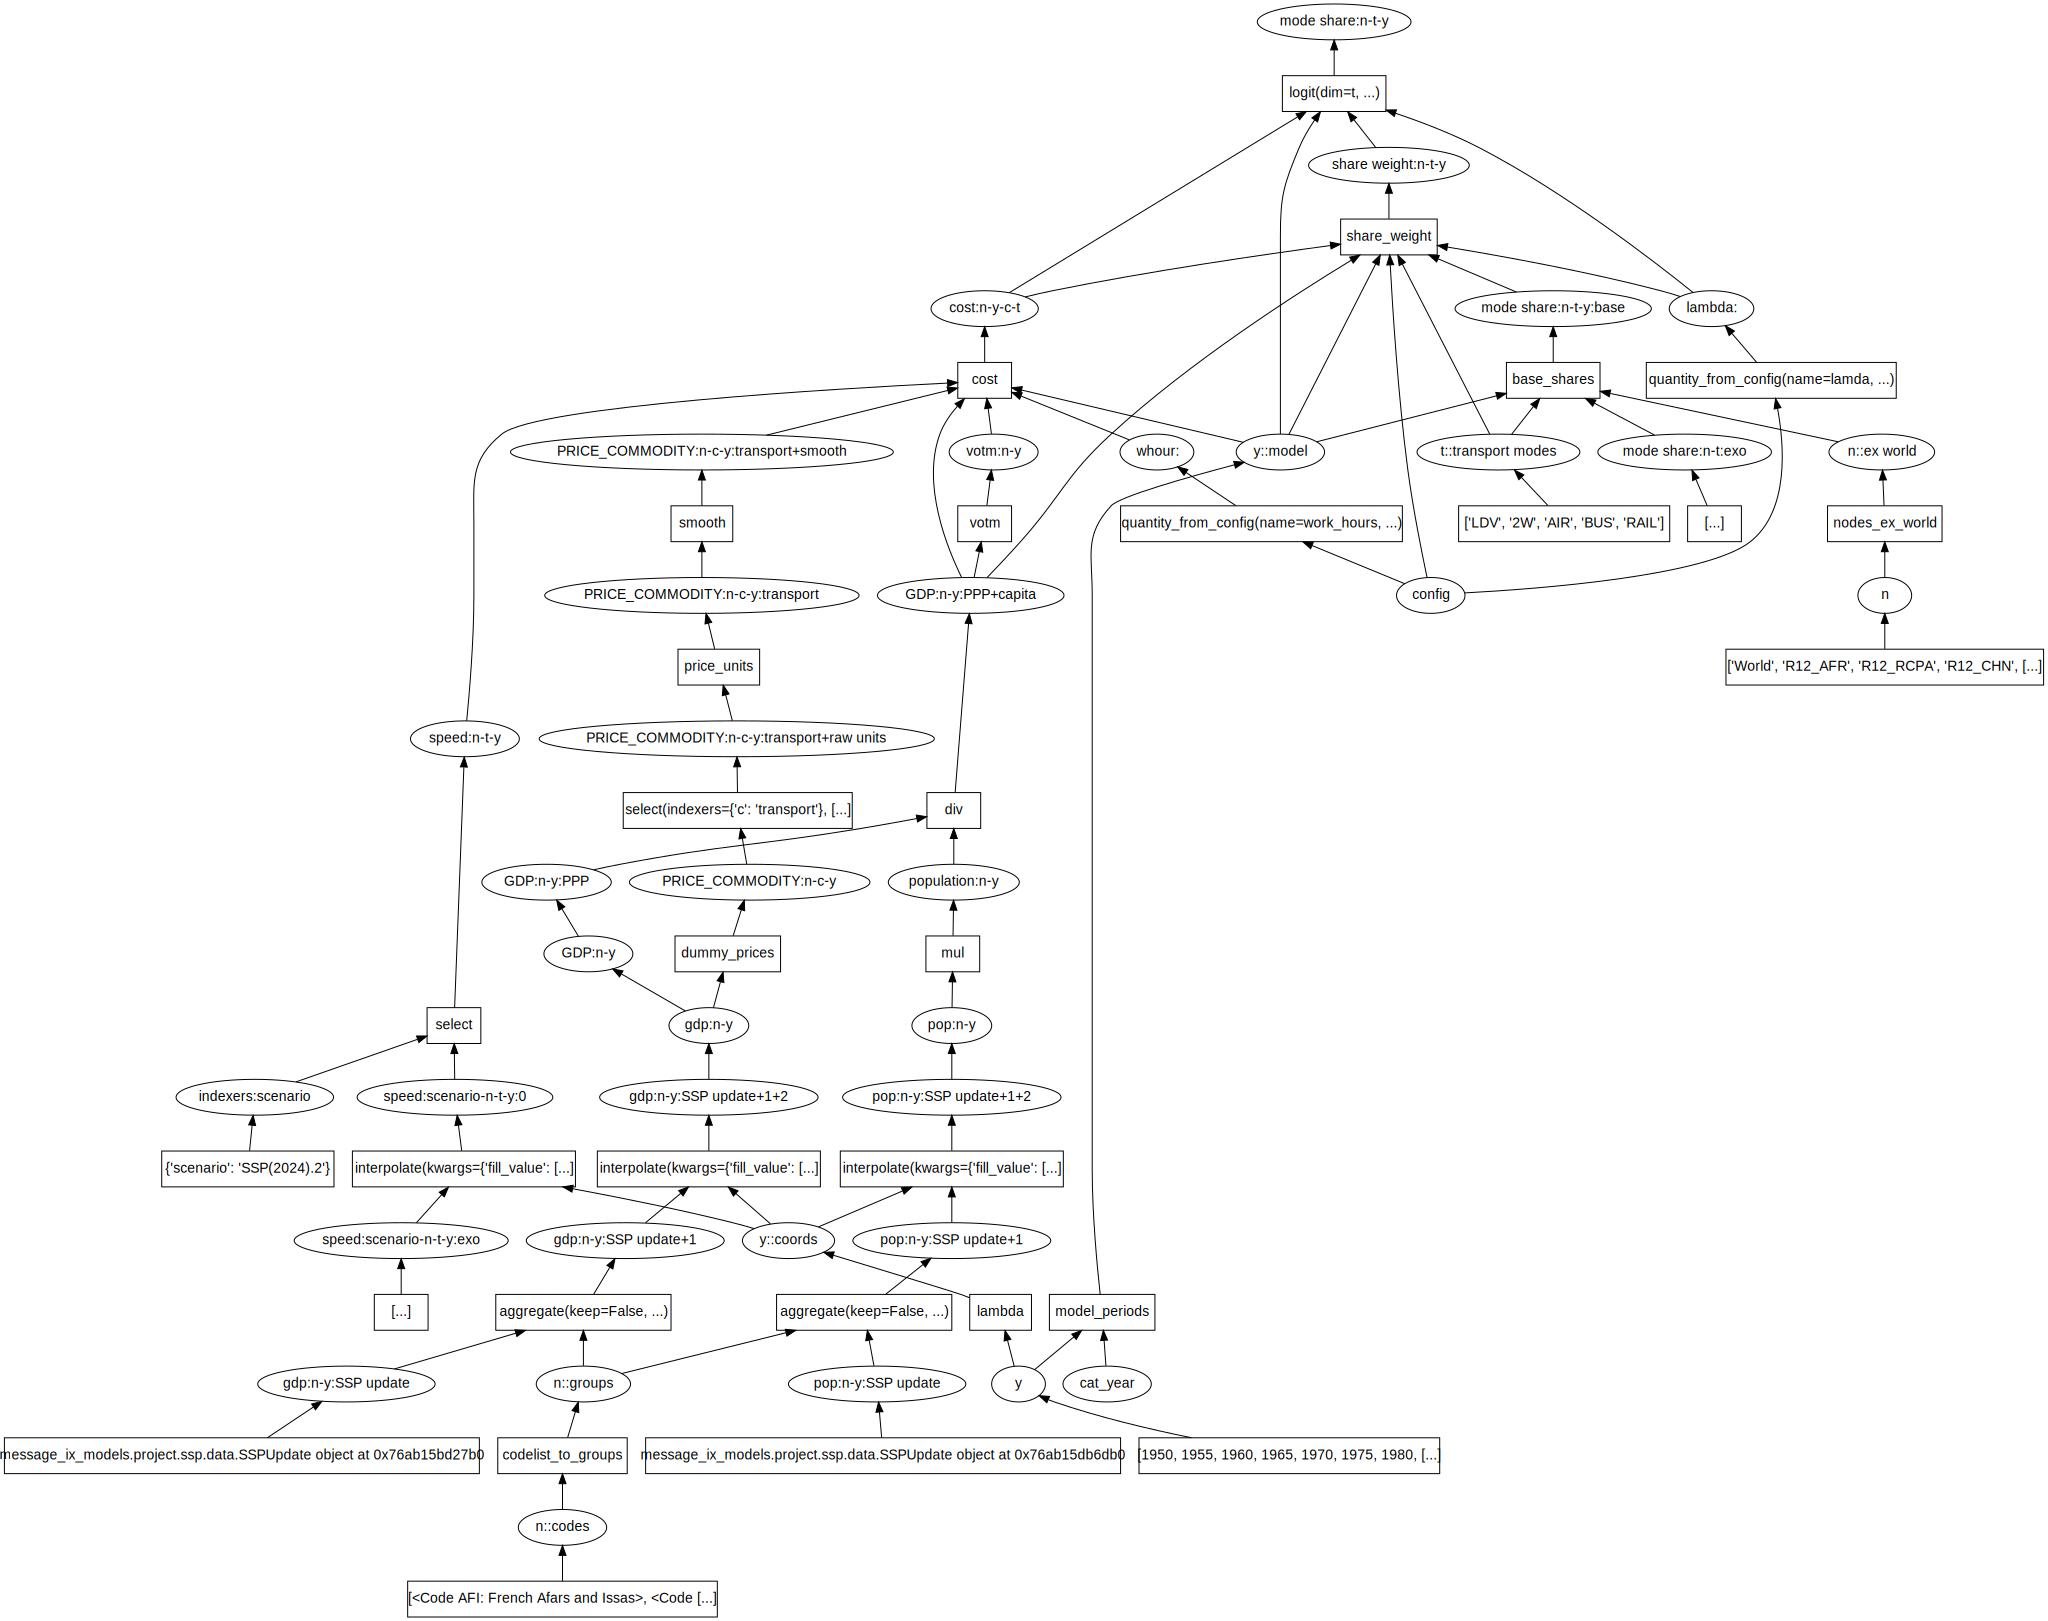
\includegraphics[width=\columnwidth]{transport-build-debug.pdf}
\column[T]{0.3\paperwidth}
\texttt{genno} makes it simple to set up \& manipulate potentially very complicated chains of these atomic steps.

\medskip
At execution, it caches and re-uses values (e.g. GDP) that flow into multiple computations, and uses \texttt{pandas} etc. for good performance.
\end{columns}
\end{frame}

\begin{frame}[fragile]
\frametitle{“Isn't this overkill? The methods are simple.”}

Often “simple methods” end up embedded 1000+-line ‘scripts’, in which are hidden bits of data, assumptions, configuration, etc.

\smallskip
Then, changing a \emph{conceptually simple} aspect of the script (e.g. add a dimension) can require an \emph{extensive rewrite}.

\bigskip
Because all intermediates are labelled in \texttt{genno}, we can simply:
\begin{enumerate}
  \item Identify a quantity to be changed or replaced.
  \item Pick the desired key, e.g. \verb@<cost:n-y-c-t>@.
  \item “Prune” off the sub-graph of tasks that yields these values.
  \item Define some other operations (load a file, do other methods) to produce a value for the same key (measure \& dimensionality).
\end{enumerate}
\end{frame}

\subsection{Ongoing work \& future directions}

\begin{frame}
\frametitle{Ongoing work \& future directions}

\begin{enumerate}
  \item “Demand-side” changes (\href{https://iiasa.ac.at/projects/edits}{EDITS project}) —replace default activity projection (based on modified logic per \textcite{schafer-2009}) with transformed data directly from ITF-OECD PASTA.
  \item Direct integration with MESSAGEix-Materials.
  \begin{itemize}
    \item Growth of vehicle \texttt{CAP} → inflows of materials used in vehicles.
    \item Growth of mode \texttt{ACT} → inflows of materials used in infrastructures.
  \end{itemize}
  \item Trip-based activity projection.
  \item Links to other, detailed models of water freight \& air transport.
\end{enumerate}

\end{frame}

\section{Shared Socioeconomic Pathways (SSPs) 2024 \& ScenarioMIP}

\subsection{Linked scenario processes}
\subsection{ScenarioMIP, CMIP7, IPCC AR7}

\begin{frame}
\frametitle{Linked scenario processes: ScenarioMIP}

\begin{columns}
\column[T]{0.425\paperwidth}
For IPCC AR7 (ca. 2028), many \structure{earth system models} will run as part of Coupled Model Intercomparison Project 7.
\begin{itemize}
  \item Same \structure{inputs} to each CM: emissions of GHGs and non-GHGs in 5–6 scenarios (right).
  \item Distinct \structure{outputs} from each CM → info about uncertainty etc.
\end{itemize}

\bigskip
ScenarioMIP = IAMs' output compared and selected for CMIP7 inputs.

\column[T]{0.425\paperwidth}
\includegraphics[width=\columnwidth]{van-vuuren-tebaldi-oneill-2023-f1.png}
DOI: \href{https://doi.org/10.5281/zenodo.8186116}{10.5281/zenodo.8186116}, Fig. 1\\
\href{https://wcrp-cmip.org/mips/scenariomip/}{wcrp-cmip.org/mips/scenariomip}
\end{columns}

\end{frame}

\begin{frame}
\frametitle{ScenarioMIP/CMIP7 timeline}
\includegraphics[width=\columnwidth]{van-vuuren-tebaldi-oneill-2023-f3.png}
DOI: \href{https://doi.org/10.5281/zenodo.8186116}{10.5281/zenodo.8186116}, Fig. 3
\end{frame}

\subsection{SSP 2024 update}

\begin{frame}[allowframebreaks]
\frametitle{SSP 2023–2024 update}
The original \structure{Shared Socioeconomic Pathways} (SSPs) were published in 2016–2017 (\textcite{riahi-2017} = overview paper).

\bigskip
These are \structure{narratives} describing 5 possible future worlds in which:
\begin{itemize}
  \item Challenges to climate change \emph{mitigation} are either small or large.
  \item Challenges to climate change \emph{adaptation} are either small or large.
\end{itemize}
…and include details about socio-economics (incl. inequality), technology, etc.

\bigskip
These narratives were \structure{realised/quantified} through:
\begin{itemize}
  \item Common demographic \emph{inputs} to IAMs: population, GDP.
  \item Several IAMs \emph{interpretation} of the narratives' meaning w.r.t. their input data and assumptions.
\end{itemize}

\framebreak
In 2023, a process started to \structure{update the SSP quantifications}.
\begin{itemize}
  \item \textbf{No change} to the narratives.
  \item Updated common socioeconomics.
  \item Updated interpretation by same IAMs, possibly more.
\end{itemize}

\bigskip
These new SSP realizations are \emph{also} used as basis for ScenarioMIP submissions:
\begin{itemize}
  \item “High” ScenarioMIP scenario may be based on an IAM's SSP5 or SSP3.
  \item “Medium” ScenarioMIP scenario may be based on SSP2.
  \item etc.
\end{itemize}

\end{frame}

\begin{frame}
\frametitle{Further details}

The ScenarioMIP emissions are \structure{not the same} as an (expected) AR7 Scenario Database (likely to be similar to the AR6 Scenario Database).
\begin{itemize}
  \item Such a database will accept many more scenarios, hopefully from a broader range of models, implementing narratives that may be different from the SSP narratives.
  \item ScenarioMIP emissions are needed because CMIP7 ESMs are big, complex, take time to run; this work must start if results are to be ready for AR7.
\end{itemize}

\bigskip
IAM teams have thus been working on 2 tasks:
\begin{enumerate}
  \item Update common GDP/pop + all other inputs/assumptions, for each SSP.
  \item Select from their 5 SSP realizations or derive further scenarios + submit to ScenarioMIP.
\end{enumerate}
\end{frame}

\subsection{Interpretation in MESSAGEix-GLOBIOM and -Transport}

\begin{frame}
\frametitle{MESSAGEix-GLOBIOM SSP update}

An updated ‘base’ version of MESSAGEix-GLOBIOM is used for SSP 2024/ ScenarioMIP.

\medskip
MESSAGEix-Transport and some other detailed variants \structure{are not used directly}.

\bigskip
Rather:
\begin{enumerate}
  \item MESSAGEix-Transport \& co. \structure{implement the SSP narratives} \emph{within} their respective sector/input data.
  \item Outputs from these detailed variants are \structure{aggregated} and used to parametrize MESSAGEix-GLOBIOM.
\end{enumerate}

\end{frame}

\begin{frame}[plain]

\vspace*{2mm}
\begin{columns}
\column[T]{0.75\paperwidth}
\includegraphics[height=\paperheight]{bauer-2017-f1.jpg}

\column[T]{0.25\paperwidth}
\bigskip
Narrative details for the energy sector in the 5 SSPs \parencite[][fig. 1]{bauer-2017}

\end{columns}
\end{frame}

\begin{frame}
\frametitle{MESSAGEix-Transport implementation of SSPs}
\framesubtitle{Some challenges}

\begin{itemize}
  \item SSP narratives are high level → there are multiple possible/consistent interpretations of how transport (sub)system(s) will change.
  \item \structure{No coordination} was planned → each modeling teams' choices will be different.
  \item SSPs are fundamentally \structure{outcome-based} → transport system changes are not represented based on epistemic/measurement uncertainty in input parameters (e.g. lowest vs. highest plausible values) but by selecting values \emph{such that} the projected outcome matches the SSP narrative.
  \item Many input parameters with high resolution → many values to set or adjust for each SSP.
\end{itemize}
\end{frame}

\begin{frame}[plain]
\hspace*{-11mm}
\includegraphics[height=\paperheight,page=1]{messageix-transport-ssp-narrative.pdf}
\end{frame}

\begin{frame}[plain]
\hspace*{-11mm}
\includegraphics[height=\paperheight,page=2]{messageix-transport-ssp-narrative.pdf}
\end{frame}

\begin{frame}
\frametitle{Following the SSP/ScenarioMIP processes}

\structure{Be critical and careful consumers} of these scenarios.
\begin{itemize}
  \item Scenarios are constructed for the specific purposes described above.
  \item They have sufficient quality from this perspective.
  \item Some value as common points for derived work that can be comparable.
  \item May not be the right starting point for exploring narratives that don't align with the SSP narratives.
\end{itemize}
\end{frame}

\makefinalslide

\appendix

\begin{frame}[allowframebreaks]
\frametitle{References}

\printbibliography[heading=none]

\end{frame}

\end{document}
